\documentclass[12pt,a4paper]{article}
\usepackage{lineno}
\usepackage{draftwatermark}
\usepackage{graphicx}
\usepackage{hyperref}

% \linenumbers
\SetWatermarkText{E L DALISTAN}
\SetWatermarkScale{3}

%%%%%%%%%%%%%%%%%%%%%%%%%%%%%%%%%%%%%%%%%%%%%%%%%%
\setlength{\topmargin}{0mm}
\setlength{\headheight}{0mm}
\setlength{\headsep}{0mm}
\setlength{\oddsidemargin}{0mm}
\setlength{\textwidth}{165mm}
\setlength{\textheight}{247mm}
\setlength{\parindent}{6pt}
\setlength{\parskip}{0pt}
%%%%%%%%%%%%%%%%%%%%%%%%%%%%%%%%%%%%%%%%%%%%%%%%%%

\begin{document}

\noindent \textbf{CE297 - HW1} \\
\textbf{Name:} \noindent Enrico Miguel Dalistan \\
\textbf{Student No.} \noindent 2011-79757\\
\bigskip
\bigskip
\bigskip

% Personal background
\noindent \textbf{1. Personal Background} \\

\noindent My first encounter with FEM is during my work as a graduate engineer.
Working with 2D plate elements, I was introduced to the concept of meshing (discretisation)
in order to arrive at more accurate results. \\

\noindent Although I acquired some intuitive understanding of the processes involved, I never had any formal academic background with the topic, especially with its
mathematical formulation until taking CE 257 from which I gained further understanding of
the method's fundamental principles. \\
\bigskip

% My Interests
\noindent \textbf{2. Interest(s)}\\

\noindent I have always been interested with the subject of Finite Element and Structural Dynamics.
Oddly enough, I was not able to fix on something considerably practical as of yet. However, I enjoyed taking courses on
both subjects which made me appreciate their beauty (FEM, especially) and appreciate the works which made
all the progress hitherto possible.\\

\noindent On the other hand, my interest in the mathematics of both subjects converges with my interests
in programming and software development. I am planning to learn more (deeply) on the theories in these subjects
to be able to write my own solutions. Furthermore, I am working with the idea of writing a Deep Learning (AI)
algorithm that could improve the efficiency of solving problems in structural mechanics
which is the central concept of my planned thesis. \\
\bigskip

% My Favourite Courses
\noindent \textbf{3. Favourite Courses}
\begin{table} [htb]
  \begin{center}
    \caption{My Courses}
    {\begin{tabular} [t] {ccc}
        \hline
        \textbf{Course Code} & \textbf{Course Title}                   & \textbf{Year Taken} \\
        \hline
        ES 204               & Numerical Methods in Engineering        & 2021                \\
        CE 226               & Structural Dynamics                     & 2021                \\
        CE 257               & Discrete Methods of Structural Analysis & 2021                \\
      \end{tabular}}
  \end{center}
\end{table}

\newpage
% Page 2

% Figure
\textbf{4. Figure - Dynamic Problem}
\begin{figure} [h]
  \begin{center}
    \scalebox{0.5}{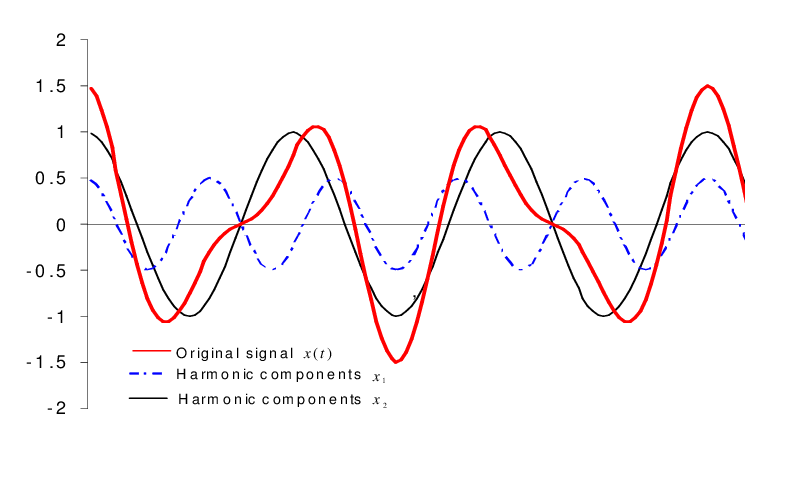
\includegraphics{./vib-signal.png}}
    \caption{Vibration signal decomposition into two harmonic components.}
    \label{image}
  \end{center}
\end{figure}
\bigskip

% Animation
\textbf{5. Animation}

\bigskip

% Equation
\textbf{6. My Favourite Equation}
\begin{equation}
  \mathbf{e}^\mathbf{ix} = \mathbf{\cos{x}} + \mathbf{i \sin{x}}
\end{equation}
\bigskip

% Schedule
\textbf{7. Available Schedule}
\begin{enumerate}
  \item Monday 2:00PM - 5:00PM
  \item Wednesday 2:00PM - 5:00PM
  \item Thursday 2:00PM - 5:00PM
\end{enumerate}
\bigskip

% ref
\noindent \textbf{References}\\
\noindent [\ref{image}] Saadat, Boulanouar \& Hafaifa, Ahmed \& Mouloud, Guemana. (2016).
Vibration analysis and measurement based on defect signal evaluation: Gas turbine investigation.
\textit{Journal of Advanced Research in Science and Technology. 3. 271-280.}\\
Available at: \href{https://www.researchgate.net/publication/311702658_Vibration_analysis_and_measurement_based_on_defect_signal_evaluation_Gas_turbine_investigation}{https://www.researchgate.net/publication/311702658}
\bigskip

\begin{center}
  \textbf{** END **}
\end{center}

\end{document}